\documentclass[11pt,a4paper]{article}

% for Chinese
%\usepackage{fontspec}  % 加這個就可以設定字體
%\usepackage[BoldFont, SlantFont]{xeCJK}  % 讓中英文字體分開設置
%\setCJKmainfont{新細明體}  % 設定中文為系統上的字型，而英文不去更動，使用原TeX\字型

% useful packages
\usepackage{amsfonts}
\usepackage{amssymb}
\usepackage{amsmath}
\usepackage{amsthm}
\usepackage{epsfig}
\usepackage{graphicx}
\usepackage{natbib}
\usepackage{textcomp}
\usepackage{booktabs}
\usepackage{multirow}
\usepackage{url}
\usepackage{color}
\usepackage{fullpage}
\usepackage[capitalize]{cleveref}
\usepackage{mathtools}
\usepackage{enumitem}
\usepackage{authblk}
\usepackage{algorithm}
\usepackage{algpseudocode}
\usepackage{subcaption}

% basic setting
\renewcommand{\baselinestretch}{1.25}
\parskip=5pt
\parindent=20pt
\footnotesep=5mm

% abbreviation
\newtheorem{lem}{Lemma}
\newtheorem{prop}{Proposition}
\newtheorem{thm}{Theorem}
\newtheorem{defn}{Definition}
\newtheorem{cor}{Corollary}
\newtheorem{assp}{Assumption}
\newtheorem{obs}{Observation}
\newenvironment{pf}{\begin{proof}\vspace{-10pt}}{\end{proof}}
% \newtheorem{ques}{Question}
% \newtheorem{rmk}{Remark}
% \newtheorem{note}{Note}
% \newtheorem{eg}{Example}

\newenvironment{enumerateTight}{\begin{enumerate}\vspace{-8pt}}{\end{enumerate}\vspace{-8pt}}
\newenvironment{itemizeTight}{\begin{itemize}\vspace{-8pt}}{\end{itemize}\vspace{-8pt}}
\leftmargini=25pt   % default: 25pt
\leftmarginii=12pt  % default: 22pt


\title{Operations Research, Spring 2024 (112-2) \\ Final Project Proposal}

\author{Ting-Hsu Chen} % r11725010@ntu.edu.tw
\author{Yuan-Ting Lin} % r11725022@ntu.edu.tw
\affil{Department of Information Management, National Taiwan University}



\begin{document}
\maketitle



\section{Introduction}
\label{sec-intro}
In this project, we collaborate with the IEDO company, which runs a car rental business 24 hours a day, 7 days a week in Taiwan by owning stations and cars of different levels. Customers can visit a station to rent or return a car and seek assistance from customer service representatives. Figure \ref{fig:cars} presents a photograph taken at a typical station, where cars of different levels are ready for rental.\footnote{Source: https://www.ctee.com.tw/news/20200110700290-431207.} Moreover, for car rental businesses to be welcomed by customers, it is crucial to open sufficient stations so that customers can conveniently access their services. Figures \ref{fig:easy_rent} and \ref{fig:car_plus} illustrate the distribution of service stations in Taipei city for two leading companies in the car rental business, Easy Rent and Car Plus, respectively.

\begin{figure}[!hbt]
\centering
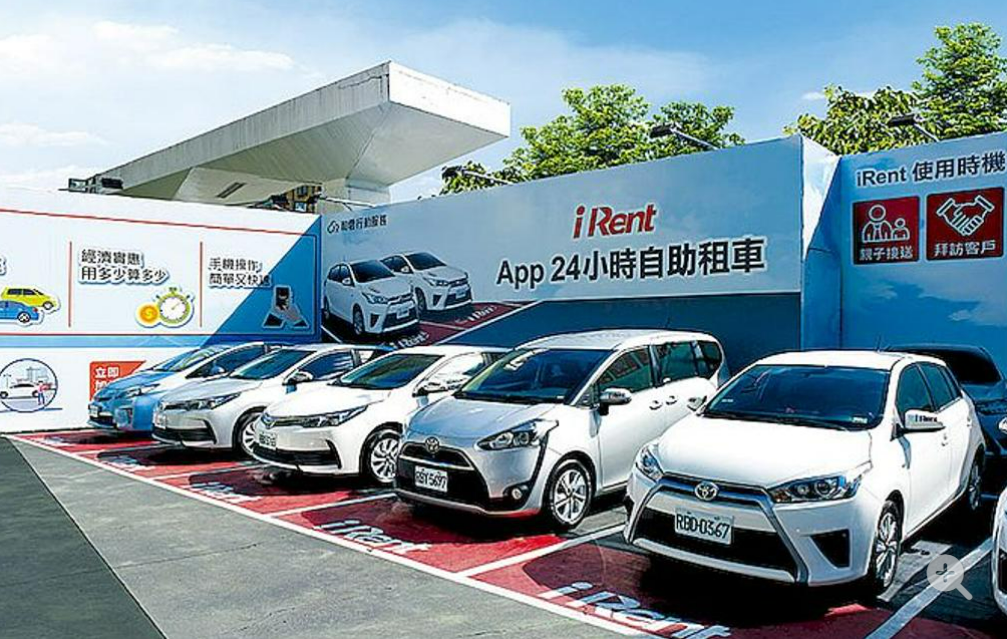
\includegraphics[width=0.7\textwidth]{figures/cars.png}
\caption{Cars of different levels offered at a station}
\label{fig:cars}
\end{figure}

\begin{figure}[!hbt]
\centering
	\begin{minipage}[b]{0.48\textwidth}
\centering
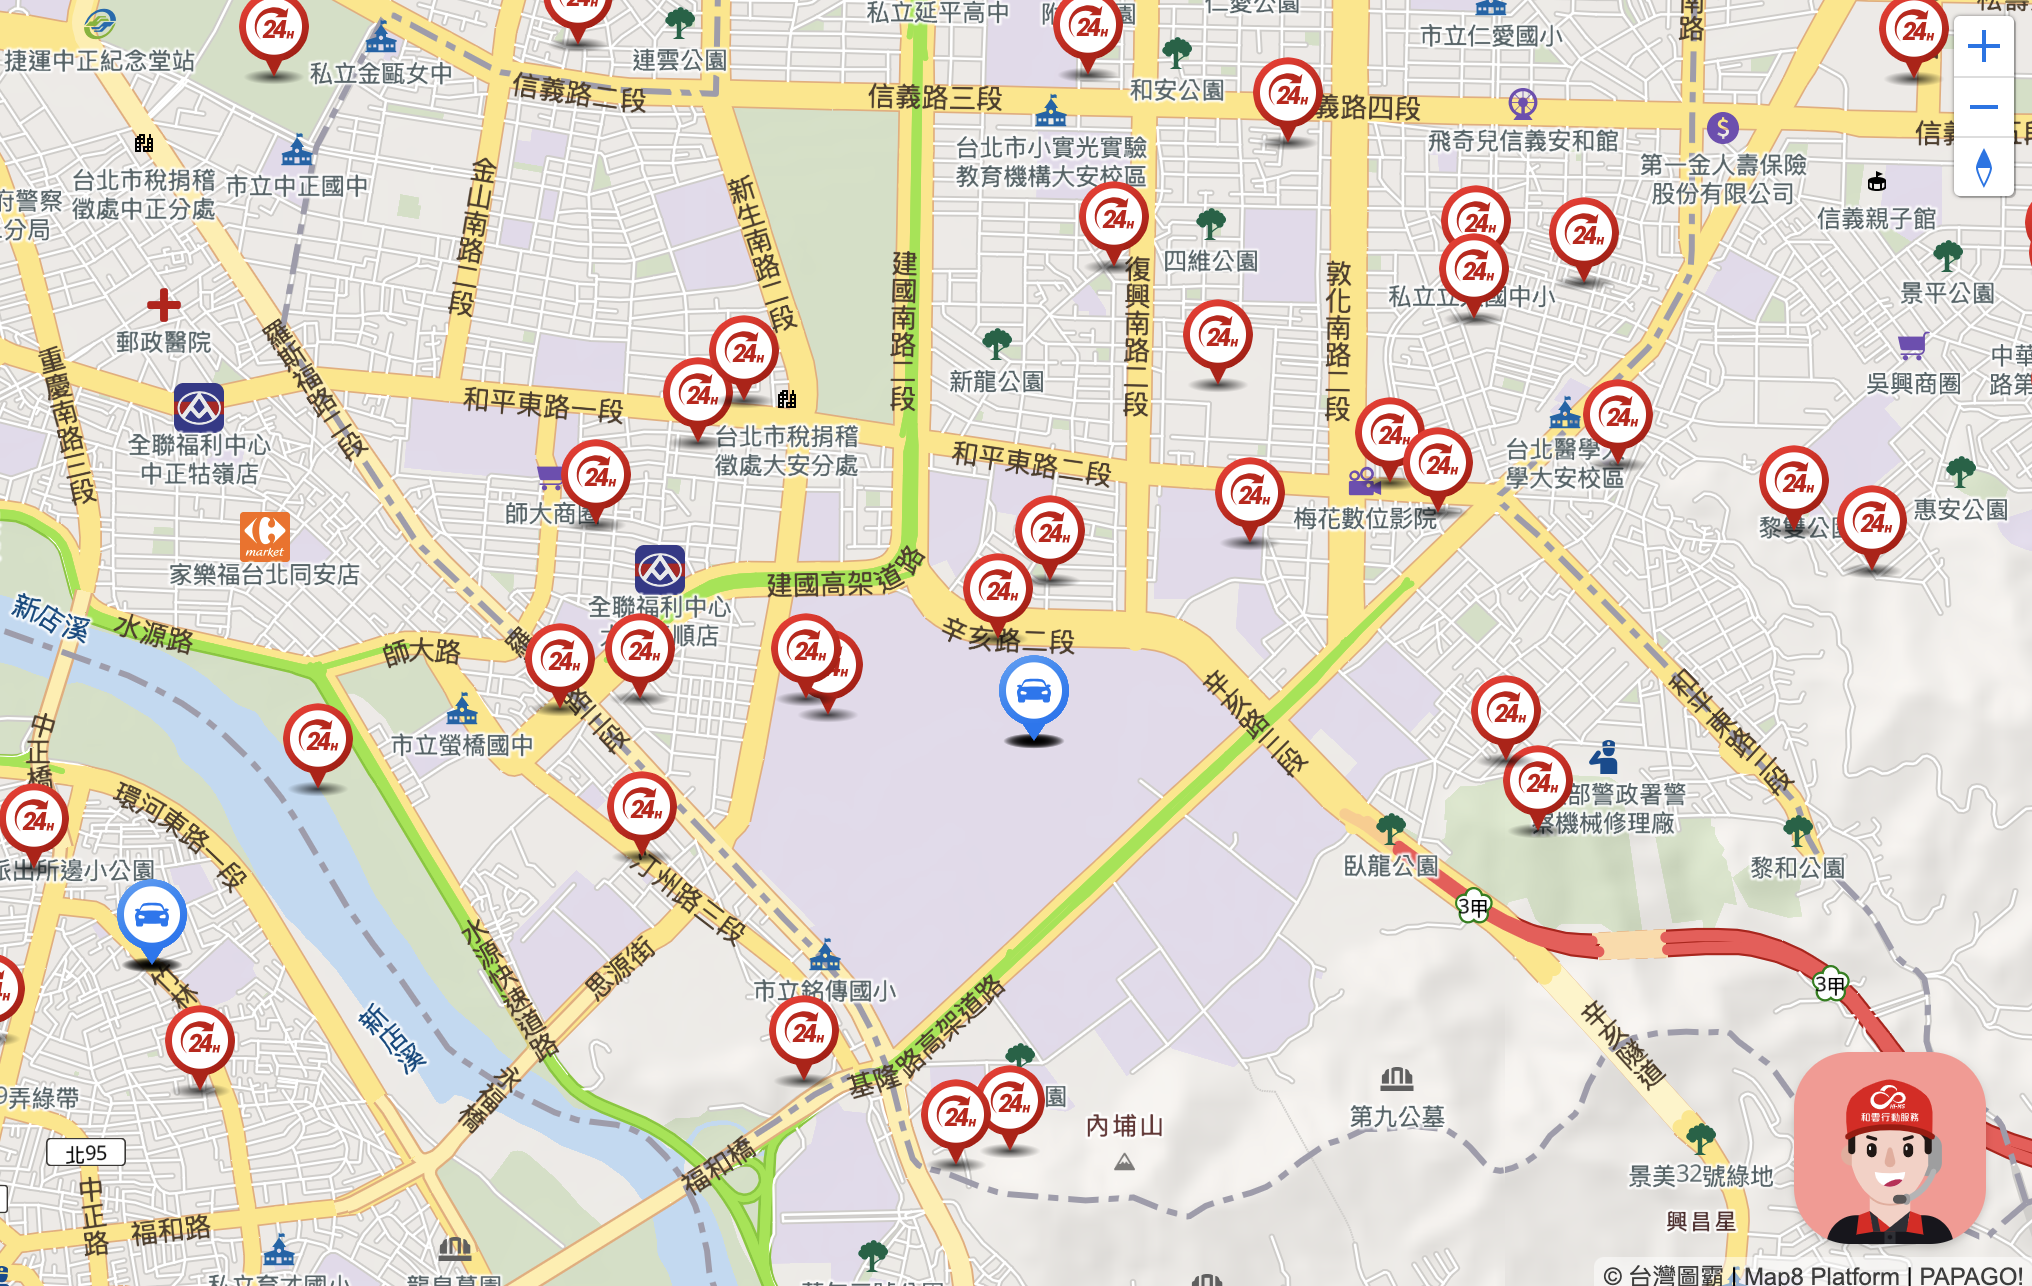
\includegraphics[width=\textwidth]{figures/easyrent.png}
\caption{Easy Rent's stations}
\label{fig:easy_rent}
	\end{minipage}
	\begin{minipage}[b]{0.01\textwidth}
		\
	\end{minipage}	
	\begin{minipage}[b]{0.48\textwidth}
\centering
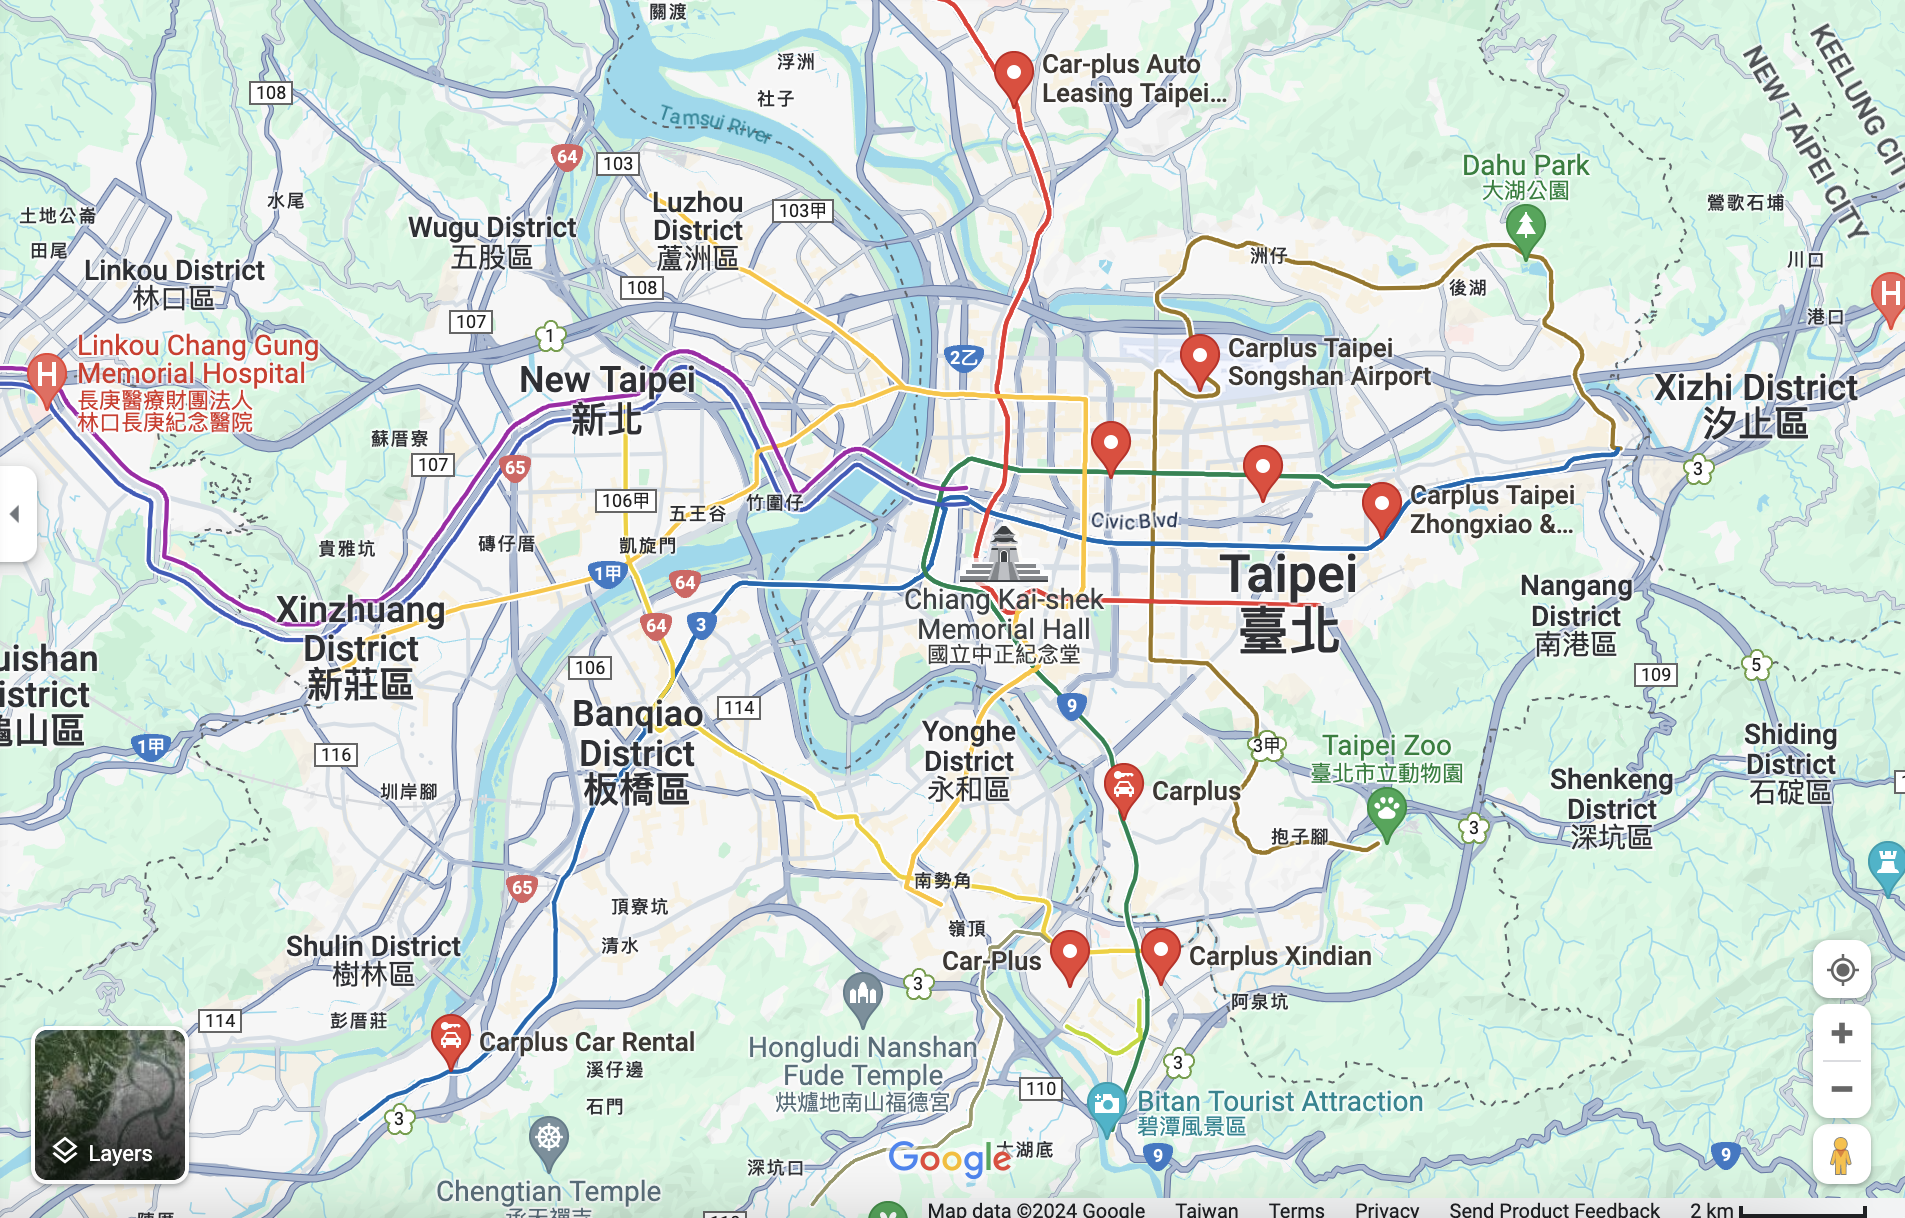
\includegraphics[width=\textwidth]{figures/carplus.png}
\caption{Car Plus' stations}
\label{fig:car_plus}
	\end{minipage}
\end{figure}

Typically, customers book cars via the IEDO company's website before they need the cars. In each order, a customer specifies (1) a car level, (2) the date, time, and station to pick up the car, and (3) the date, time, and station to return the car. The car rental fee, which is also the revenue earned by the IEDO company by fulfilling the order, is also specified. The pick-up station and return station are allowed to be different in an order. 

To handle customer orders, the IEDO company divides its decision process into two stages. In the first stage, the IEDO company has to determine whether to \textit{accept} an order received from its website. The decision is based on a set of empirical rules, such as checking whether the total number of requested cars exceeds those available during a specific period. While these rules are designed by experienced managers, they may sometimes accept too many orders that not all orders are likely to be fulfilled in practice. 

Because there are many accepted orders, it is possible that cars are not enough at some stations in some periods. Therefore, in the second stage of the decision process, the IEDO company must consider rearranging cars by having its employees move cars among stations or provide free upgrades to \textit{fulfill} orders. The IEDO company collects revenue from an order if it is fulfilled. However, if it fails to fulfill an accepted order, resulting in customer dissatisfaction and inconvenience, it will not only fail to earn revenue from the order but also need to compensate the customers.

To resolve the above issue, while integrating the two-stage decision process into a single stage (i.e., considering all the decisions simultaneously) may be the best solution, modifying the rules specified in the first stage requires a huge amount of effort to communicate with high-level managers. Therefore, the IEDO company has chosen to prioritize addressing the second-stage problem. To maximize the total profit as well as to maintain the level of customer satisfaction, it is imperative to generate an effective rearrangement and upgrade plan. 
If the IEDO company fails to handle the orders effectively, customers may find its service inconvenient and unreliable, and they may decide to patronize other competitors instead. This challenge becomes even more difficult during peak seasons, which requires the IEDO company to manage thousands of orders, hundreds of cars, and tens of stations. 

Currently, the rearrangement and upgrade plan is computed by two experienced managers using pencil and paper. However, they have to spend two whole days figuring out a plan for the orders for the upcoming week. Though the plan they generated seems not too bad, the IEDO company has difficulty evaluating the quality of the plan and is interested in whether there are better approaches to address the second-stage problem both efficiently and effectively.

In this project, we try to help the IEDO company figure out the above problem. We assume the first-stage decisions have been made and fixed, and a set of accepted orders is given. Our primary goal is to address the second-stage problem by designing a planning approach to make a rearrangement and upgrade plan according to given conditions to maximize the IEDO company's total profit. Additionally, since we focus on the second-stage problem only, in the sequel, we will refer to ``accepted orders'' as ``orders'' when there is no ambiguity. 










\section{Problem description}
\label{sec-problem}

Given the orders in a certain period, the IEDO company has to find out a rearrangement and upgrade plan to fulfill the orders.
The planning horizon expands from 00:00 of the first day to 24:00 of the last day. It is assumed that all cars will be picked up on time, and a car to be rented must be ready at the station thirty minutes earlier than the pick-up time (e.g., if a customer books a car at 10:00 at station 1, the car must be ready at station 1 at 9:30 or earlier).\footnote{By the way, the abbreviation of ``for example'' in English is ``e.g.,'', not ``ex'' or ``ex:'' or whatever.}

The IEDO company assumes that customers will always return cars on time. Right after a car is returned, the car will be cleaned by the employees at the return station. The cleaning time required depends on the return time of the car. For example, when a car is returned between 08:00 and 12:00 or between 14:00 and 18:00, the cleaning time is one hour. However, there is a lunch break from 12:00 to 14:00, so if a car is returned within this period, it will have to wait and be cleaned after the break. The car will thus finish the cleaning process at 15:00 as the cleaning time is also one hour. Moreover, most employees get off work at 18:00. Due to a staff shortage from 18:00 to 08:00 of the next day, the cleaning process will take three hours when the car is returned within this period. Table \ref{tab:cleaning_time} summarizes the cleaning time required for different return times.

\begin{table}[!hbt]
\centering
\begin{tabular}{c|c}
\toprule
Return time & Cleaning time required \\
\midrule
    08:00--12:00 & 1 hour \\
    12:00--14:00 & 1 hour after 14:00 \\
    14:00--18:00 & 1 hour \\
    18:00--08:00 & 3 hours \\
\bottomrule
\end{tabular}
\caption{Cleaning time required for different return times}
\label{tab:cleaning_time}
\end{table}

After the cleaning process, a car is considered ready. A car may be moved to another station by an IEDO employee only after it is cleaned. It is assumed that all cars are ready and may be picked up by a customer right away at the beginning moment of the planning horizon. 

To fulfill orders to earn revenues as much as possible, the IEDO company should allow cars to be moved among stations. As we mentioned above, a car may be moved from a station only after it has been cleaned. The traveling time to move a car from station to station satisfies the triangular inequality. Moreover, it is known that the outbound travel time is the same as the inbound travel time between all pairs of stations. As the IEDO company does not have an unlimited number of employees, the total amount of time spent on moving all cars cannot exceed a predetermined number. Furthermore, it is assumed that as long as the total moving time is within the predetermined upper limit, there is a reasonable way to find enough employees to execute the plan. We also assume that the parking lots at any station are unlimited. 

An alternative way to fulfill more orders is to provide upgrades. The IEDO company allows an order asking for a car of a certain level to be satisfied by and only by a car with the same level or the one with only a level higher. Even though upgrades are free, this may still help the IEDO company earn more revenues by fulfilling more low-level orders with spare high-level cars.

While car rearrangements and upgrades may help the IEDO company fulfill more orders, it is still possible that some orders are not being fulfilled. Therefore, the planning process needs to determine three things: (1) which orders to fulfill, (2) whether free upgrades should happen for each order, and (3) when and from where to where to move cars.

If an order is fulfilled, the IEDO company collects a corresponding sales revenue. The sales revenue is computed as the hourly rate, which depends on the car level requested by the order, multiplied by the number of hours a car is rented in the order. If in the end an order cannot be fulfilled and must be rejected, the IEDO company pays the customer half of the order's price to compensate the customer's loss. The IEDO company's objective of planning is to maximize its total profit, which is the total sales revenue minus the total compensation, for the orders in the planning horizon.










\section{Mathematical model}
\label{sec-model}

In this section, we formulate a mixed linear integer program to precisely describe our problem presented in Section \ref{sec-problem}.

Let $I = \{1, ..., n_C\}$ be the set of cars, and $L = \{1, ..., n_L\}$ be the set of car levels. Level $l_1$ is considered as a lower level than level $l_2$ if $l_1 < l_2$. All cars in the same level are considered the same. Moreover, let $K = \{0, 1, ..., n_K\}$ be the set of orders, where 0 is a virtual order that is scheduled at the first and the last positions on each car to ensure that for each non-virtual order, there is exactly one predecessor and one successor. We define the return station of order 0 on car $i$ as the initial station of car $i$. In the sequel, we use $i$ as the index of cars and $j$ and $k$ as the indices of orders.

To assign orders to cars, let the decision variable $x_{ik} \in \{0, 1\}$ be 1 if the demand of order $k$ is satisfied by car $i$ or 0 otherwise. If order $k$ is fulfilled, the IEDO company earns $R_k = F_l H_k$ dollars as its sales revenue, where $F_l$ is the hourly rate of a level-$l$ car, and $H_k$ is the number of hours a car is rented in order $k$. The IEDO company pays $0.5R_k$ to compensate the customer if order $k$ cannot be fulfilled and must be rejected. With these notations, the total cost that the IEDO company seeks to minimize is then
\begin{align}
    \min \quad & \sum_{k \in K \setminus \{0\}} \left(R_k \Big(\sum_{i \in I} x_{ik}\Big) - 0.5R_k \Big(1 - \sum_{i \in I} x_{ik}\Big)\right) \label{obj-maxRevenue}.
\end{align}

In addition to assigning a car to satisfy the demand of an order, the sequence of orders on the same car should also be determined. Let $y_{ijk} \in \{0, 1\}$ be 1 if order $k$ is scheduled right after order $j$ on car $i$ or 0 otherwise. An order $k$ can be scheduled after another order $j$ on car $i$ only if the car levels asked by orders $j$ and $k$ match the level of car $i$ (upgrade considered), and the length of the period between the return time of order $j$ and the pick-up time of order $k$ is sufficient (for cleaning, possible car rearranging, and being ready). Let $A_{ijk}$ be 1 if order $k$ can be scheduled after order $j$ on car $i$ or 0 otherwise. Note that $A_{ijk}$ is a parameter and is readily available once the information of car $i$ and orders $j$ and $k$ are provided. The constraints that ensure a feasible car-order assignment is
\begin{align}
    & \sum_{i \in I} x_{ik} \leq 1 \quad \forall k \in K \setminus \{0\} \label{constr-accepted} \\
    & y_{ijk} \leq A_{ijk} \quad \forall i \in I, j \in K, k \in K \label{constr-avaliable}.
\end{align}
Constraint (\ref{constr-accepted}) ensures that each non-virtual order will be assigned to at most one car. Constraint (\ref{constr-avaliable}) set $y_{ijk}$ to 0 if order $k$ cannot be scheduled after order $j$ on car $i$ ($A_{ijk} = 0$).
 
There are more constraints for the sequence of orders on a car. Initially, the order sequence of each car begins with a virtual order, which is followed by at most one real order. Moreover, if an order is allocated to a car, there should be an order (virtual order included) preceding it and another order (virtual order included) succeeding it. We then have
\begin{align}
    & \sum_{k \in K \setminus \{0\}} y_{i0k} \leq 1 \quad \forall i \in I \label{constr-initial} \\
    & \sum_{k \in K} y_{ijk} = x_{ij} \quad \forall i \in I, j \in K \setminus \{0\} \label{constr-xy01} \\
    & \sum_{j \in K} y_{ijk} = x_{ik} \quad \forall i \in I, k \in K \setminus \{0\} \label{constr-xy02}
\end{align}
Constraint (\ref{constr-initial}) ensures the virtual order on each car is followed by at most one real order. Constraint (\ref{constr-xy01}) ensures that when order $j$ is fulfilled by car $i$, i.e., $x_{ij} = 1$, there should be exactly one order succeeding order $j$, and thus $\sum_{k \in K} y_{ijk} = 1$. When $x_{ij} = 0$, which implies $\sum_{k \in K} y_{ijk} = 0$, there should be no order adjacent to order $j$ on car $i$. The meaning of constraint (\ref{constr-xy02}) is similar to constraint (\ref{constr-xy01}). 

To address rearrangement, we use $T_{ijk}$ to denote the amount of time required to move car $i$ from the return station of order $j$ to the pick-up station of order $k$, and let $B$ be the limit of the total amount of time spent on moving all cars. The budget constraint of  rearranging cars is then
\begin{align}
    & \sum_{i \in I} \sum_{j \in J} \sum_{k \in \setminus \{0\}} T_{ijk}y_{ijk} \leq B \label{constr-limit}.
\end{align}
The LHS of constraint (\ref{constr-limit}) computes the total amount of time relocating all cars, which cannot exceed the predetermined limit $B$.

To complete the formulation, we finally add 
\begin{align}
    & x_{ik} \in \{0,1\} \quad \forall i \in I, k \in K  \label{constr-binary-x} \\
    & y_{ijk} \in \{0,1\} \quad 
    \forall i \in I, j \in K, k \in K, \label{constr-binary-y}
\end{align}
which are the binary constraints of the decision variables.










\section{Expected results}
\label{sec-expected}

To approach our problem, we will first collect relevant data provided by the IEDO company, including information on orders, cars, and stations. For data that are not available from the IEDO company, we will randomly generate them according to the estimated distribution of the real-world situation faced by the IEDO company. Moreover, we will write a computer program to calculate the values of parameters required for our mathematical program from the raw data. 

For small-scale instances, we plan to implement the mixed linear integer programming model by writing a Python program that invokes Gurobi Optimizer to obtain an optimal rearrangement and upgrade plan. For large-scale instances, finding an optimal solution may be too time-consuming and thus not practical; therefore, we seek to develop a heuristic algorithm that can generate near-optimal solutions efficiently. To demonstrate the effectiveness of our algorithm, we will conduct case studies to compare our solution approach with the current approach adopted by the IEDO company, some very naive heuristics, and some upper bound of an optimal solution. Furthermore, extended experiments will be performed to evaluate the robustness of our algorithm through various scenarios. Finally, we will provide some closing remarks to conclude our study.

\end{document}
